\chapter{Стороны}\label{ENTITIES}

\section{Перечень сторон}

Cторона ИОК характеризуется уникальными идентификационными данными.
%
Cторона владеет одной или несколькими парами ключей (личным и открытым),
каждой из которой соответствует сертификат, выпущенный в ИОК. 
%
Идентификационные данные стороны повторяются во всех ее сертификатах.
%
%Сторона может обновить сертификат, сохранив ключевую пару 
%(см.~\ref{PROCESSES.Reenroll}). 

Несколько сертификатов может потребоваться стороне при взаимодействии 
с различными прикладными системами. В разных контекстах взаимодействия
сторона может выступать в разных ролях, 
использовать ключи разных уровней стойкости (см.~\ref{CRYPTO.Params}), 
управлять различными цифровыми ресурсами (см.~\ref{ENTITIES.SAN}). 
%
\addendum{
Кроме этого, логически единая сторона может состоять из нескольких 
компонентов, каждый из которых имеет собственную пару ключей 
и соответствующий сертификат. При этом во всех сертификатах указываются 
единые идентификационные данные.
%
Например, СШВ может представлять собой масштабируемый набор физических серверов, 
которые выпускают штампы времени от общего имени, используя собственные личные ключи.
}

Подчинение стороны~$A$ стороне~$B$ означает, что~$A$ получила сертификат 
у~$B$: $A$ является субъектом сертификата, $B$~--- эмитентом.
%
\addendum{Речь идет о логическом подчинении в рамках ИОК.
Подчинение не означает, что~$A$ является подразделением~$B$ или сотрудником~$B$. 
Более того, подчиненная сторона~$A$ может представлять ту же организацию, 
что и~$B$.
%
Создание в пределах одного ЮЛ нескольких сторон ИОК, возможно 
подчиненных друг другу, может использоваться для конкретизации сфер 
полномочий и обязанностей.
%
Например, от РУЦ может быть логически отделен ПУЦ, 
отвечающий только за выпуск сертификатов для КТ.
}

Стороны ИОК делятся на УЦ, которые могут выпускать сертификаты открытых ключей, 
и конечных участников, которые выпускать сертификаты не могут.

В ИОК поддерживается следующая иерархия: 
имеется единственный КУЦ (точка доверия), единственный РУЦ и
произвольное число ПУЦ. РУЦ подчиняется КУЦ, ПУЦ подчиняется РУЦ. 
Сертификаты конечным участникам выдает либо РУЦ, либо ПУЦ.
В первом случае участника связывает с КУЦ цепочка сертификатов длины 3,
во втором~--- длины 4.

Определены следующие роли конечных участников ИОК:
\begin{enumerate}
\item
ЦАС. Подчиняется РУЦ либо одному из ПУЦ. 
Выпускает атрибутные сертификаты для 
конечных участников, обслуживаемых некоторым (не обязательно своим) УЦ.
Правила функционирования ЦАС определены в СТБ 34.101.67.

\item
РЦ. Подчиняется РУЦ.
Является посредником при взаимодействии между конечными участниками и УЦ:
проводит первичную аутентификацию, регистрирует идентификационные данные,
организует подготовку запросов на получение сертификата, визирует запросы. 
%
Для аутентификации и сбора идентификационных данных может 
взаимодействовать с КТ пользователей, выступая в качестве терминала. 
%  
РЦ обслуживает один или несколько УЦ. Может дополнительно 
обслуживать СИ, регистрируя данные или устройства для аутентификации 
(например, пароль или КТ). 

\item
OCSP-сервер. Подчиняется РУЦ, либо одному из ПУЦ.
По запросам сторон выпускает справки (OCSP-ответы)
о текущем статусе сертификатов, выданных своим УЦ. 
В роли OCSP-сервера может выступать сам УЦ.
Правила функционирования OCSP-сервера определены в СТБ 34.101.26.
%
Форматы запроса и ответа профилируется в~\ref{FMT.OCSP}.

\item
СШВ. Подчиняется РУЦ.
По запросам сторон выпускает штампы времени, которые демонстрируют 
существование определенных данных к определенному моменту времени. 
Правила функционирования СШВ определены в СТБ 34.101.82.
%
Формат штампов времени профилируется в~\ref{FMT.TSP}.

\item
СЗД. Подчиняется РУЦ.
По запросам сторон выпускает справки (аттестаты заверения)
о действительности ЭД. 
%
СЗД может проверять действительность ЭД в одной инфраструктуре и 
выпускать аттестат заверения в другой. Для проверки аттестата не нужно 
иметь доступ к первой инфраструктуре и, таким образом, СЗД позволяет 
организовать взаимодействие между сторонами инфраструктур, выступая в роли 
посредника между ними. 
%
Правила функционирования СЗД определены в СТБ 34.101.81.
Используется только один из четырех сервисов СЗД~---
сервис vsd (проверка действительности ЭД).
%
Формат аттестатов заверения профилируется в~\ref{FMT.DVCS}.

\item
СИ. Подчиняется РУЦ, либо одному из ПУЦ.
Проводит аутентификацию пользователей и, в случае успеха, выдает билеты~---
подписанные или секретные данные, которые открывают доступ пользователям к 
ресурсам прикладных систем или прикладным системам к ресурсам пользователей.
Для организации аутентификации может взаимодействовать с КТ пользователя,
выступая в качестве терминала.

\item
TLS-сервер. Подчиняется РУЦ.
Является частью прикладной системы, организует ее взаимодействие 
с другими сторонами по защищенным TLS-соединениям. 
Правила функционирования TLS-сервера описаны в СТБ 34.101.65.

\item
ФЛ. Получает сертификат в РУЦ, либо в одном из ПУЦ.
Может быть как резидентом, так и нерезидентом Республики Беларусь.

\item
ЮП. Получает сертификат в РУЦ, либо в одном из ПУЦ.
\addendum{
Представляет ЮЛ, несет ответственность за выполнение определенных процессов. 
%
Может быть оператором ПУД, подотчетного ЮЛ.
Оператор должен получать сертификаты напрямую в~РУЦ.
}

\item
КА. Получает сертификат в РУЦ, либо в одном из ПУЦ.
%
\addendum{
Может быть агентом ПУД, участвуя, например, в выпуске сертификатов.}
\end{enumerate}

УЦ может быть подчинено не более одного OCSP-сервера.
СШВ и СЗД единственны (они подчинены РУЦ). 

Стороны ИОК представлены на рисунке~\ref{Fig.ENTITIES.1}.
Роли, помеченные на рисунке звездочкой, могут быть представлены 
несколькими сторонами. Двойная линия означает однозначное соответствие 
между сторонами. Буква T означает, что сторона может выступать в качестве 
терминала. Скругленными прямоугольниками обозначены УЦ, наклоненными~--- службы.

\begin{figure}[bht]
\begin{center}
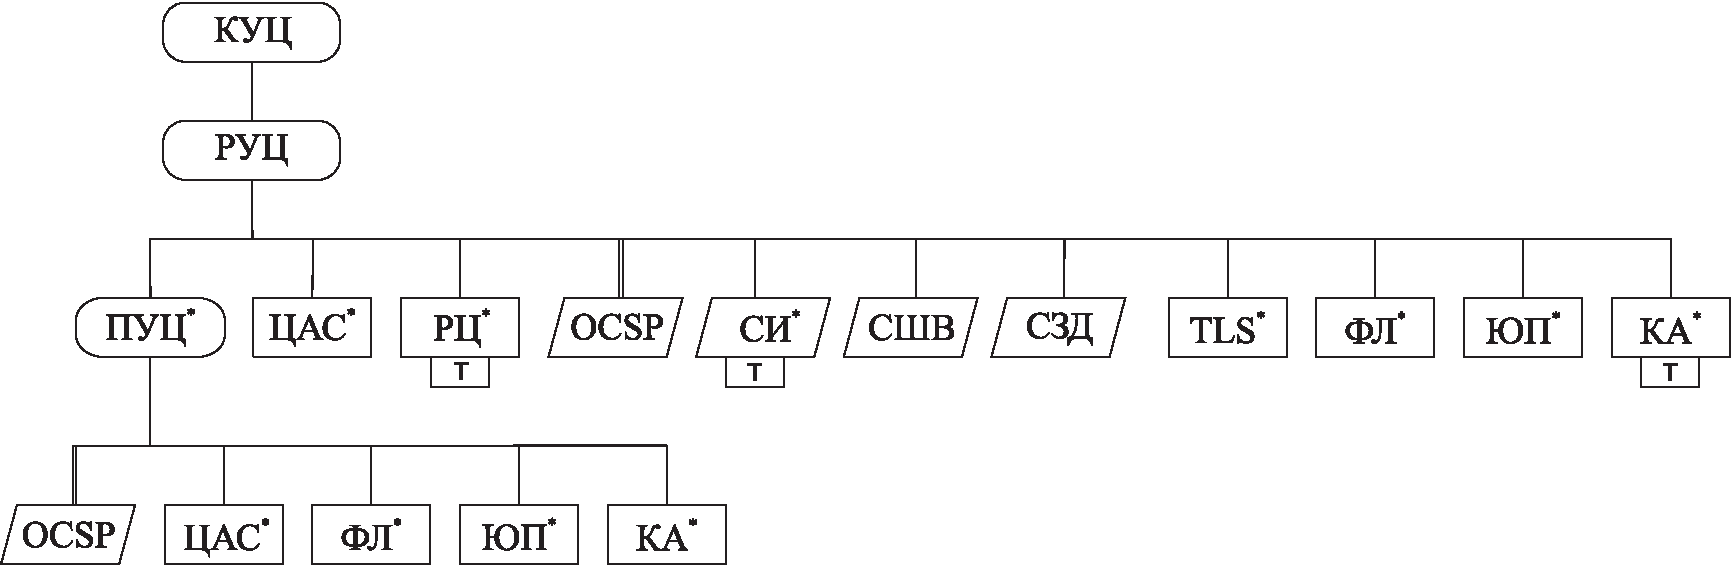
\includegraphics[width=17cm]{../figs/entities}
\end{center}
\caption{Стороны ИОК}
\label{Fig.ENTITIES.1}
\end{figure}

Ролям назначаются идентификаторы АСН.1, определенные в приложении~\ref{ASN1}. 
Идентификаторы имеют вид \verb|{bpki-role n}|,
где \verb|bpki-role|~--- префикс, определенный в приложении,
\texttt{n}~--- числовой код, заданный в таблице~\ref{Table.ENTITIES.Roles}.

В таблице полужирным шрифтом выделены роли ПУД.
Этим ролям зарезервирован диапазон кодов от~0 до~49.

Операторам ПУД назначается два идентификатора роли: 
идентификатор ЮП (основной) и идентификатор ПУД. 
%
Агентам ПУД также назначается два идентификатора: 
идентификатор КА (основной) и идентификатор ПУД. 
%
\addendum{
Дополнительный идентификатор ПУД имеет техническое значение
и не меняют принадлежности оператора роли ЮП и принадлежности агента
роли КА.}

Идентификаторы ролей конечных участников указываются в 
расширении~\texttt{CertificatePolicies} их сертификатов
(см.~\ref{FMT.Ext.CP}).

\begin{table}[bht]
\caption{Роли сторон}
\label{Table.ENTITIES.Roles}
\begin{tabular}{|l|c||l|c|}
\hline
Роль & Код & Роль & Код\\
\hline
\hline
{\bf КУЦ}        & 0    & {\bf СЗД}      & 32 \\
{\bf РУЦ}        & 1    & {\bf СИ}       & 33 \\
{\bf ПУЦ}        & 2    & TLS-сервер     & 50 \\
{\bf ЦАС}        & 10   & ФЛ-резидент    & 60 \\
{\bf РЦ}         & 20   & ФЛ-нерезидент  & 61 \\
{\bf OCSP-сервер}& 30   & ЮП             & 62 \\
{\bf СШВ}        & 31   & КА             & 70 \\
\hline
\end{tabular}
\end{table}

\section{Идентификационные данные}\label{ENTITIES.Name}

\subsection{Идентификационные атрибуты}\label{ENTITIES.Attrs}

Идентификационные данные стороны представляют собой совокупность атрибутов: 
фамилия, имя и отчество, страна, адрес, место работы и др.  
%
Атрибут описывается типом~\texttt{AttributeTypeAndValue}, определенным в 
СТБ 34.101.19, и представляет собой пару <<идентификатор~--- значение>>. 
Идентификатор атрибута определяет его семантику, 
значение описывается строкой АСН.1 определенного типа с определенными 
ограничениями на длину.  

Атрибуты укладываются в контейнер типа~\texttt{Name}. Тип также определен в 
СТБ 34.101.19. Перечень атрибутов контейнера определяется ролью идентифицируемой 
стороны. В контейнере не должно быть нескольких однотипных атрибутов.

Тип~\texttt{Name} имеют компоненты~\texttt{subject} и~\texttt{issuer} 
сертификата. Первый компонент описывает идентификационные данные субъекта, 
второй~--- эмитента.

Компонент~\texttt{subject} типа~\texttt{Name} включается также в запрос на 
получение сертификата. Указанные в компоненте идентификационные данные
заверяются РЦ в процессе выпуска сертификата. Субъект не может изменить 
данные при самостоятельном (без участия РЦ) обновлении сертификата. 

Перечень допустимых идентификационных атрибутов задан в 
таблице~\ref{Table.ENTITIES.Attrs}. Перечень составлен в соответствии 
с~СТБ 34.101.19 и~\cite{X520}.  

\begin{table}[bht]
\caption{Идентификационные атрибуты}
\label{Table.ENTITIES.Attrs}
\begin{tabular}{|l|l|l|}
\hline
Атрибут & Идентификатор & Тип значения\\
\hline
\hline
\texttt{commonName} & \verb|{2 5 4 3}| & \texttt{UTF8String(SIZE (1..64))}\\
\texttt{surname} & \verb|{2 5 4 4}| & \texttt{UTF8String(SIZE (1..128))}\\
\texttt{name} & \verb|{2 5 4 41}| & \texttt{UTF8String(SIZE (1..1024))}\\
\texttt{givenName} & \verb|{2 5 4 42}| & \texttt{UTF8String(SIZE (1..128))}\\
\texttt{serialNumber} & \verb|{2 5 4 5}| & \texttt{PrintableString(SIZE (1..64))}\\
\texttt{countryName} & \verb|{2 5 4 6}| & \texttt{PrintableString(SIZE (2))}\\
\texttt{localityName} & \verb|{2 5 4 7}| & \texttt{UTF8String(SIZE (1..128))}\\
\texttt{stateOrProvinceName} & \verb|{2 5 4 8}| & \texttt{UTF8String(SIZE (1..128))}\\
\texttt{organizationName} & \verb|{2 5 4 10}| & \texttt{UTF8String(SIZE (1..64))}\\
\texttt{organizationalUnitName} & \verb|{2 5 4 11}| & \texttt{UTF8String(SIZE (1..64))}\\
\texttt{title} & \verb|{2 5 4 12}| & \texttt{UTF8String(SIZE (1..64))}\\
\texttt{organizationIdentifier} & \verb|{2 5 4 97}| & \texttt{UTF8String(SIZE (1..64))}\\
\hline                                      
\end{tabular}
\end{table}

\if 0
issue#17: -=
\texttt{streetAddress} & \verb|{2 5 4 9}| & \texttt{UTF8String(SIZE (1..128))}\\
\fi

\begin{table}[bht]
\caption{Идентификационные атрибуты ролей}
\label{Table.ENTITIES.AttrRole}
\begin{tabular}{|l|c|c|c|c|c|c|c|}
\hline
Атрибут & \multicolumn{2}{|c|}{ПУД} & TLS- & 
\multicolumn{2}{|c|}{ФЛ} & ЮП & КА\\
\cline{2-3}
\cline{5-6}
& КУЦ & другие & сервер & резидент & нерезидент & & \\
\hline
\hline
\texttt{commonName} & 
+ & + & + & + & + & + & +\\
\texttt{surname} & 
  &   &   & + & + & + &  \\
\texttt{name} & 
  & + & + &   &   & + &  +\\
\texttt{givenName} & 
  &   &   & + & + & + &  \\
\texttt{serialNumber} & 
  &   &   & + & + & + & +\\
\texttt{countryName} & 
+ & + & + & + & + & + & +\\
\texttt{localityName} & 
  & + & + &   &   & + & +\\
\texttt{stateOrProvinceName} & 
  & $\pm$ & $\pm$ &   &   & $\pm$ & $\pm$\\
\texttt{organizationName} & 
  & + & + &   &   & + & +\\
\texttt{organizationalUnitName} & 
  & $\pm$ & $\pm$ &   &   & $\pm$ & $\pm$\\
\texttt{title} & 
  &   &   &   &   & + & \\
\texttt{organizationIdentifier} & 
  & + & + &   &   & + & +\\
\hline                                      
\end{tabular}
\end{table}

\if 0
issue#17: -= 
\texttt{streetAddress} & 
  & + & + &   &   & + & +\\
\fi

В таблице~\ref{Table.ENTITIES.AttrRole} определяются атрибуты,
которые должны быть включены в идентификационные данные сторон 
различных ролей. Пропуск в таблице означает отсутствие атрибута,
плюc~--- обязательное включение, $\pm$~--- включение при наличии.

Атрибуты~\addendum{должны быть} заданы в контейнере~\texttt{Name} в том же 
порядке, в котором они представлены в таблице~\ref{Table.ENTITIES.AttrRole}.

\addendum{В сертификатах, издаваемых ПУЦ, могут указываться дополнительные 
атрибуты.} 

\subsection{Атрибут \texttt{commonName}}\label{ENTITIES.Id.CN}

В атрибуте~\texttt{commonName} задается общее (универсальное) имя стороны.
В общем имени должны использоваться только графические символы базовой 
таблицы КОИ-7, определенной в ГОСТ 27463: латинские буквы, 
знаки препинания и базовые специальные знаки.
 
Общее имя следует выбирать так, чтобы оно кратко 
и при этом максимально однозначно характеризовало сторону. 
При выборе имени должны учитываться следующие ограничения:
\begin{enumerate}
\item
Общее имя КУЦ полагается равным \str{BY Root CA}.
\item
Общее имя РУЦ полагается равным \str{BY Republican CA}.
\item
Общее имя СШВ полагается равным \str{BY Republican TSA}.
\item
Общее имя СЗД полагается равным \str{BY Republican DVCS}.
\item
Общее имя TLS-сервера содержит единичное или подстановочное (со звездочкой) 
DNS-имя. Примеры имен: \str{www.example.org}, \str{example.org}, \str{*.example.org}.
%
Общее имя должно дублироваться в расширении \texttt{SubjectAltName} 
сертификата. В этом расширении могут быть указаны и другие DNS-имена.
\item
Общее имя ФЛ или ЮП~--- это его имя и фамилия на английском языке в 
соответствии с удостоверением.
Имя и фамилия записываются в верхнем регистре, разделяются пробелом.
Например, \str{VICTOR MITSKEVICH}.
\end{enumerate}

\subsection{Атрибут \texttt{surname}}\label{ENTITIES.Id.S}

В атрибуте~\texttt{surname} задается фамилия ФЛ или ЮП.
Фамилия задается в соответствии с удостоверением лица,
записывается прописными буквами.

Для ФЛ-резидентов и ЮП \texttt{surname} содержит белорусскую и русскую 
формы фамилии, разделенные наклонной чертой (как в паспорте).
Например, \str{МІЦКЕВІЧ/МИЦКЕВИЧ}.

% issue#3: подчеркнуть кодировку белорусских символов.

\begin{note} 
Примечание~--- Коды белорусских и русских символов определяются 
в соответствии с~\cite{UTF8}. Код символа~--- это два октета,
которые обычно записываются в шестнадцатеричной форме с префиксом
\texttt{U-}. Например, \texttt{U-0406}~--- код белорусского символа І.
Для сравнения, идентичный по начертанию латинский символ I 
задается другим кодом: \texttt{U-0049}.
%
В настоящем стандарте белорусские и русские символы 
всегда размещаются в строках типа \texttt{UTF8String}.
%
При этом символы дополнительно кодируются по правилам UTF-8, также 
определенным в~\cite{UTF8}. Кодирование UTF-8 организовано так, что 
белорусские и русские символы снова представляются двумя октетами, 
а латинские символы~--- только одним.
\end{note}

\subsection{Атрибут \texttt{name}}\label{ENTITIES.Id.N}

В атрибуте~\texttt{name} задается полное название организации
в соответствии с ее удостоверением. Например, \str{Открытое акционерное 
общество "Вектор"}.  

Здесь и далее речь идет об организации,
которая владеет ПУД или TLS-сервером, 
об организации, которая эксплуатирует КА,
или об организации, которую представляет ЮП.

\subsection{Атрибут \texttt{givenName}}\label{ENTITIES.Id.GN}

В атрибуте~\texttt{givenName} задается личное имя ФЛ или ЮП.
Личное имя уточняет идентификацию лица на основе его фамилии.
%
Имя задается в соответствии с удостоверением лица, 
записывается прописными буквами. 

Для ФЛ-резидентов и ЮП \texttt{givenName} содержит белорусскую и русскую 
формы имени и отчества. Имя и отчество разделяются пробелом, формы 
разделяются символом~\str{/} (графический код байта $47=\hex{2F}$ 
согласно базовой таблице КОИ-7). 
Например, \str{ВIКТАР АНТОНАВIЧ/ВИКТОР АНТОНОВИЧ}.

\subsection{Атрибут~\texttt{serialNumber}}\label{ENTITIES.Id.SN}

В атрибуте~\texttt{serialNumber} задается либо идентификационный номер ФЛ 
или ЮП, либо серийный номер КА. 

Строка, описывающая идентификационный номер, содержит (слева направо):
\begin{enumerate}
\item
Три символа типа номера:
\str{PAS}~--- номер паспорта, 
\str{PNO}~--- личный номер, 
\str{IDC}~--- номер id-карты.

\item
Два символа кода страны, в которой зарегистрирован номер 
(см.~\ref{ENTITIES.Id.C}).
\item
Символ \str{-} (графический код байта $45=\hex{2D}$).
\item
Собственно символы номера.
\end{enumerate}

Примеры: \str{PASBY-MP0112358}, 
\str{PNOBY-786545091A4PB5}, 
\str{IDCBE-590082394654}.

Серийный номер КА следует задавать так, чтобы он однозначно 
характеризовал оборудование КА. Например, в качестве серийного номера 
может выступать MAC-адрес сетевого устройства или IMEI-номер мобильного 
телефона. 

\subsection{Атрибут~\texttt{countryName}}\label{ENTITIES.Id.C}

В атрибуте~\texttt{countryName} задается двухбуквенный код страны
в соответствии с~\cite{CountryCodes}. 
%
Для ФЛ-нерезидента это код страны, гражданином которой он является.
Во всех остальных случаях код полагается равным~\str{BY}.

\subsection{Атрибуты адреса}\label{ENTITIES.Id.L}

В атрибутах~\texttt{localityName} и~\texttt{stateOrProvinceName} 
задается информация из юридического адреса организации,
которая владеет ПУД или TLS-сервером, или организации, 
которую представляет ЮП.
%
Адрес задается в соответствии с удостоверением организации. 

В атрибуте~\texttt{localityName} указывается населенный пункт:
город (\str{г.}), городской поселок (\str{г.п.}), 
деревня (\str{д.}) и др.
%
% поселок (\str{п.}), агрогородок (\str{а.г.})?
%
Примеры: \str{г.~Каменец}, \str{д.~Каменюки}.

\if 0
issue#17: -=
В атрибуте \texttt{streetAddress} указываются следующие реквизиты:
название улицы (проспекта, бульвара, переулка), номер дома, 
номер корпуса (строения), номер квартиры (кабинета, помещения, офиса). 
Реквизиты приводятся в порядке их объявления, разделяются запятыми. 
Ненужные реквизиты опускаются. 
%
Примеры: 
\str{ул.~Снежная, д.~1, корп.~1, кв.~2},
\str{3-й пер. Морозный, д.~5}.
\fi

В атрибуте~\texttt{stateOrProvinceName} указываются названия области и района.
Атрибут не включается в идентификационные данные, если в~\texttt{localityName}
указан областной центр.
В атрибуте опускается название района, если в~\texttt{localityName}
указан районный центр.
Примеры: 
\str{Брестская обл., Каменецкий р-н} (для \str{д.~Каменюки}),
\str{Брестская обл.} (для \str{г.~Каменец}).

\subsection{Атрибут \texttt{organizationName}}\label{ENTITIES.Id.O}

В атрибуте~\texttt{organizationName} задается сокращенное название организации,
которая владеет ПУД или TLS-сервером, или организации, которую 
представляет ЮП.
%
Сокращенное название задается в соответствии с удостоверением организации. 
Например, \str{ОАО "Вектор"}.  

\subsection{Атрибут \texttt{organizationalUnitName}}\label{ENTITIES.Id.OU}

В атрибуте~\texttt{organizationalUnitName} может задаваться название 
подразделения организации, которая отвечает за управление ПУД или TLS-сервером, 
или подразделения, которое представляет ЮП.
%
Название подразделения задается в соответствии с удостоверением 
организации. Например, \str{отдел цифровых технологий}. 

\subsection{Атрибут \texttt{title}}\label{ENTITIES.Id.T}

В атрибуте~\texttt{title} задается должность ЮП в организации, которую он 
представляет. 
%
Должность задается в соответствии с удостоверением ЮП. Например, 
\str{начальник отдела}.   

\subsection{Атрибут \texttt{organizationIdentifier}}\label{ENTITIES.Id.ORGID}

В атрибуте~\texttt{organizationIdentifier} задается идентификатор организации,
которая владеет ПУД или TLS-сервером, или организации, которую 
представляет ЮП.

Строка, описывающая идентификатор, содержит (слева направо):
\begin{enumerate}
\item
Три символа типа идентификатора.
Разрешается использовать только код 
\str{TAX}~--- учетный номер плательщика.

\item
\str{BY}~--- код страны, в которой зарегистрирован идентификатор.

\item
Символ \str{-}.
\item
Собственно символы идентификатора.
\end{enumerate}

Пример: \str{TAXBY-235831459}.

\section{Дополнительные идентификационные данные}\label{ENTITIES.SAN}

В расширении \texttt{subjectAltName} сертификата могут быть указаны 
дополнительные идентификационные данные. Эти данные представляют собой 
совокупность атрибутов, описывающих цифровые ресурсы стороны. 
%
Атрибуты задаются в компонентах вложенного в~\texttt{subjectAltName} 
типа~\texttt{GeneralName}. Тип определен в СТБ 34.101.19.
%
Перечень допустимых атрибутов задается таблицей~\ref{Table.ENTITIES.AttrsEx}. 

\begin{table}[bht]
\caption{Дополнительные идентификационные атрибуты}
\label{Table.ENTITIES.AttrsEx}
\begin{tabular}{|l|p{8.9cm}|l|}
\hline
Атрибут & Семантика (примеры) & Компонент \texttt{GeneralName}\\
\hline
\hline
\texttt{email} & 
адрес электронной почты (\url{alice@example.org}) & 
\verb|rfc822Name|\\
%
\texttt{DNS} & 
DNS-имя (\url{www.example.org}, \texttt{*.example.org}) &
\verb|dNSName|\\
%
\texttt{URI} & 
URI (\url{http://example.org/responder}) &
\verb|uniformResourceIdentifier|\\
%
\texttt{IP} & 
IP-адрес (93.184.216.34) &
\verb|iPAddress|\\
\hline                                      
\end{tabular}
\end{table}

В расширении \texttt{subjectAltName} должен присутствовать хотя бы один 
идентификационный атрибут. Может присутствовать несколько атрибутов одного 
типа. Общее число атрибутов не должно быть больше~\addendum{$100$}.

TLS-сервер должен указать в расширении \texttt{subjectAltName}
все свои DNS-имена. СШВ, СЗД и СИ \addendum{могут} указать в расширении 
URI своих узлов.

Расширение \texttt{subjectAltName} включается в запрос на получение сертификата 
и переносится из запроса в сертификат. При обработке запроса РЦ или УЦ 
могут проверять владение ресурсами, которые описываются атрибутами расширения. 
%
Способ проверки определяется вне рамок настоящего стандарта.

Дополнительные идентификационные атрибуты \addendum{могут быть} 
изменены при самостоятельном (без участия РЦ) обновлении сертификата.

